\documentclass[journal,12pt,twocolumn]{IEEEtran}

\usepackage{setspace}
\usepackage{gensymb}
\singlespacing
\usepackage[cmex10]{amsmath}

\usepackage{amsthm}

\usepackage{mathrsfs}
\usepackage{txfonts}
\usepackage{stfloats}
\usepackage{bm}
\usepackage{cite}
\usepackage{cases}
\usepackage{subfig}

\usepackage{longtable}
\usepackage{multirow}

\usepackage{enumitem}
\usepackage{mathtools}
\usepackage{steinmetz}
\usepackage{tikz}
\usepackage{circuitikz}
\usepackage{verbatim}
\usepackage{tfrupee}
\usepackage[breaklinks=true]{hyperref}
\usepackage{graphicx}
\usepackage{tkz-euclide}

\usetikzlibrary{calc,math}
\usepackage{listings}
    \usepackage{color}                                            %%
    \usepackage{array}                                            %%
    \usepackage{longtable}                                        %%
    \usepackage{calc}                                             %%
    \usepackage{multirow}                                         %%
    \usepackage{hhline}                                           %%
    \usepackage{ifthen}                                           %%
    \usepackage{lscape}     
\usepackage{multicol}
\usepackage{chngcntr}

\DeclareMathOperator*{\Res}{Res}

\renewcommand\thesection{\arabic{section}}
\renewcommand\thesubsection{\thesection.\arabic{subsection}}
\renewcommand\thesubsubsection{\thesubsection.\arabic{subsubsection}}

\renewcommand\thesectiondis{\arabic{section}}
\renewcommand\thesubsectiondis{\thesectiondis.\arabic{subsection}}
\renewcommand\thesubsubsectiondis{\thesubsectiondis.\arabic{subsubsection}}


\hyphenation{op-tical net-works semi-conduc-tor}
\def\inputGnumericTable{}                                 %%

\lstset{
%language=C,
frame=single, 
breaklines=true,
columns=fullflexible
}
\begin{document}


\newtheorem{theorem}{Theorem}[section]
\newtheorem{problem}{Problem}
\newtheorem{proposition}{Proposition}[section]
\newtheorem{lemma}{Lemma}[section]
\newtheorem{corollary}[theorem]{Corollary}
\newtheorem{example}{Example}[section]
\newtheorem{definition}[problem]{Definition}

\newcommand{\BEQA}{\begin{eqnarray}}
\newcommand{\EEQA}{\end{eqnarray}}
\newcommand{\define}{\stackrel{\triangle}{=}}
\bibliographystyle{IEEEtran}
\raggedbottom
\setlength{\parindent}{0pt}
\providecommand{\mbf}{\mathbf}
\providecommand{\pr}[1]{\ensuremath{\Pr\left(#1\right)}}
\providecommand{\qfunc}[1]{\ensuremath{Q\left(#1\right)}}
\providecommand{\sbrak}[1]{\ensuremath{{}\left[#1\right]}}
\providecommand{\lsbrak}[1]{\ensuremath{{}\left[#1\right.}}
\providecommand{\rsbrak}[1]{\ensuremath{{}\left.#1\right]}}
\providecommand{\brak}[1]{\ensuremath{\left(#1\right)}}
\providecommand{\lbrak}[1]{\ensuremath{\left(#1\right.}}
\providecommand{\rbrak}[1]{\ensuremath{\left.#1\right)}}
\providecommand{\cbrak}[1]{\ensuremath{\left\{#1\right\}}}
\providecommand{\lcbrak}[1]{\ensuremath{\left\{#1\right.}}
\providecommand{\rcbrak}[1]{\ensuremath{\left.#1\right\}}}
\theoremstyle{remark}
\newtheorem{rem}{Remark}
\newcommand{\sgn}{\mathop{\mathrm{sgn}}}
\providecommand{\abs}[1]{\left\vert#1\right\vert}
\providecommand{\res}[1]{\Res\displaylimits_{#1}} 
\providecommand{\norm}[1]{\left\lVert#1\right\rVert}
%\providecommand{\norm}[1]{\lVert#1\rVert}
\providecommand{\mtx}[1]{\mathbf{#1}}
\providecommand{\mean}[1]{E\left[ #1 \right]}
\providecommand{\fourier}{\overset{\mathcal{F}}{ \rightleftharpoons}}
%\providecommand{\hilbert}{\overset{\mathcal{H}}{ \rightleftharpoons}}
\providecommand{\system}{\overset{\mathcal{H}}{ \longleftrightarrow}}
	%\newcommand{\solution}[2]{\textbf{Solution:}{#1}}
\newcommand{\solution}{\noindent \textbf{Solution: }}
\newcommand{\cosec}{\,\text{cosec}\,}
\providecommand{\dec}[2]{\ensuremath{\overset{#1}{\underset{#2}{\gtrless}}}}
\newcommand{\myvec}[1]{\ensuremath{\begin{pmatrix}#1\end{pmatrix}}}
\newcommand{\mydet}[1]{\ensuremath{\begin{vmatrix}#1\end{vmatrix}}}
\numberwithin{equation}{subsection}
\makeatletter
\@addtoreset{figure}{problem}
\makeatother
\let\StandardTheFigure\thefigure
\let\vec\mathbf
\renewcommand{\thefigure}{\theproblem}
\def\putbox#1#2#3{\makebox[0in][l]{\makebox[#1][l]{}\raisebox{\baselineskip}[0in][0in]{\raisebox{#2}[0in][0in]{#3}}}}
     \def\rightbox#1{\makebox[0in][r]{#1}}
     \def\centbox#1{\makebox[0in]{#1}}
     \def\topbox#1{\raisebox{-\baselineskip}[0in][0in]{#1}}
     \def\midbox#1{\raisebox{-0.5\baselineskip}[0in][0in]{#1}}
\vspace{3cm}
\title{EE3025 ASSIGNMENT- 1}
\author{Ritwik Sahani - EE18BTECH11038}
\maketitle
\newpage
\bigskip
\renewcommand{\thefigure}{\theenumi}
\renewcommand{\thetable}{\theenumi}
Download all python codes from 
\begin{lstlisting}
https://github.com/ritvix23/EE3025-IDP-DSP/tree/main/Assignment1/codes
\end{lstlisting}
And Latex-tikz codes from - 
\begin{lstlisting}
https://github.com/ritvix23/EE3025-IDP-DSP/tree/main/Assignment1
\end{lstlisting}

%

\section{Problem}
    
The command
\begin{lstlisting}
    output_signal = signal.lfilter(b,a,output_signal)
\end{lstlisting}
in Problem 2.3 is executed through following difference equation 
    \begin{align} \label{eq:ProblemEqn}
        \sum _{m=0}^{M}a\brak{m}y\brak{n-m}=\sum _{k=0}^{N}b\brak{k}x\brak{n-k}
    \end{align}
 where input signal is $x(n)$ and output signal is $y(n)$ with intial values all 0. Replace \textbf{signal.filtfilt} with your own routine and verify
  \section{Solution}
  This can be done using two different algorithms. Let us discuss both of them one by one.
  
  \subsection{Algorithm 1}
  A simple way could be to implement literally what equation \ref{eq:ProblemEqn} does, that is, find the output sequence sample by sample using previously calculated samples. However, the in-built routine \textbf{signal.filtfilt} does more than this. Upon checking the official documentation, it turns out that the in-built routine implements a forward-backward filter. So, let's first understand what a forward-backward filter is and why we need it.
  
  \subsubsection{Forward-Backward Filter}
  When we apply a filter, say a third order lowpass Butterworth filter, to an input signal, the filter introduces a phase lag at the output. This was the forward application of the filter, in a sense that we applied the filter to the input sequence just the way it was. In order to nullify this phase lag, we apply the same filter again at the output sequence obtained after forward pass, but after inverting the output sequence in time domain. This is the backward pass. The output from the backward pass is inverted again to give the final output of the forward-backward filter. The following equations should make it clear mathematically - 
  \begin{align}
      v\brak{n}=\brak{h*x}\brak{n}
  \end{align}
  here, $v\brak{n}$ is the ouptput of the first filtering operation, namely the forward pass, $x\brak{n}$ is the input sequence, $h\brak{n}$ is the filter impulse response. For the backward pass we invert/flip $v\brak{n}$, so say $v$ = [1, 2, 3], $FLIP\brak{v}$  = [3, 2, 1]. Now, 
  \begin{align} 
      w\brak{n}=\brak{h*FLIP\brak{v}}\brak{n}
  \end{align}
  $w\brak{n}$ is the output sequence from the second pass. It is inverted again to get final output - 
  \begin{align}\label{eq:Forward-Backward_eqn}
      y\brak{n}=\brak{FLIP\brak{w}}\brak{n}
  \end{align}

  As we discussed earlier, one straight-forward algorithm to implement this filtering procedure is to use loops and calculate each output sample one by one. Rearranging equation \ref{eq:ProblemEqn} as -
  \begin{align}
        a\brak{0}y\brak{n}=\sum _{k=0}^{N}b\brak{k}x\brak{n-k} - \sum _{m=1}^{M}a\brak{m}y\brak{n-m}
    \end{align}
    \begin{align} \label{eq:Modified_eqn}
        y\brak{n}=\frac{\sum _{k=0}^{N}b\brak{k}x\brak{n-k} - \sum _{m=1}^{M}a\brak{m}y\brak{n-m}}{a\brak{0}}
    \end{align}
  Arrays can be used to store past N+1 samples of input signal and past M samples of output signal, and these can be updated iteratively.
  \\
  The soundfile generated from this algorithm can be found at - 
  \begin{lstlisting}
https://github.com/ritvix23/EE3025-IDP-DSP/tree/main/Assignment1/soundfiles/Sound_from_algo1.wav
  \end{lstlisting}
  \subsection{Algorithm 2}
  Another way could be to convert the sequences to z-domain, apply corresponding operations, and convert back.
  \\
  Let' continue from equation \ref{eq:Forward-Backward_eqn} as - 
  \begin{align}
    y\brak{n}=\brak{FLIP\brak{w}}\brak{n}
  \end{align}
  \begin{align}
    y\brak{n}=FLIP\brak{h*FLIP\brak{h*x}}\brak{n}
  \end{align}
  Take z-transform both sides - 
  \begin{align} \label{eq: z_relation}
    Y\brak{Z}=H(z^{-1})H\brak{z}X\brak{z}
  \end{align}
  Where we used, 
  \begin{align}
        {\mathcal{Z}}\{h\} = H\brak{z} \\
      \implies{\mathcal{Z}}\{FLIP\brak{h}\} = H(z^{-1})
  \end{align}
  $H\brak{z}$ can be obtained by taking z-transform both sides in equation \ref{eq:ProblemEqn}, 
  \begin{align}
     Y\brak{z} \sum _{m=0}^{M}a\brak{m} z^{-m} = X\brak{z} \sum _{k=0}^{N}b\brak{k}z^{-k}
\end{align}
\begin{align}
\label{eq:Hz_eqn}
    H\brak{z} = \frac{Y\brak{z}}{X\brak{z}} = \frac{\sum _{k=0}^{N}b\brak{k} z^{-k}}{\sum _{m=0}^{M}a\brak{m}z^{-m}}
\end{align} 
 Where we used,
  \begin{align}
      {\mathcal {Z}}\{x(n-k)\} = z^{-k}X(z) \\
      {\mathcal {Z}}\{y(n-m)\} = z^{-m}Y(z)
  \end{align}
 The above algorithm can be implemented using built-in \textbf{fft} command to convert sequences to z-domain, and \textbf{ifft} command to convert them back to time domain.
 \\
 The soundfile generated from this algorithm can be found at- 
 \begin{lstlisting}
https://github.com/ritvix23/EE3025-IDP-DSP/tree/main/Assignment1/soundfiles/Sound_from_algo2.wav
 \end{lstlisting}
 The soundfile generated from builtin routine can be found at- 
 \begin{lstlisting}
https://github.com/ritvix23/EE3025-IDP-DSP/tree/main/Assignment1/soundfiles/Sound_from_builtin_routine.wav
 \end{lstlisting}
 Single code file containing both the above algorithms can be found at - 
 \begin{lstlisting}
https://github.com/ritvix23/EE3025-IDP-DSP/tree/main/Assignment1/codes/ee18btech11038.py
 \end{lstlisting}
 
\section{Comparison}
Algorithm 1 takes $O\brak{L\brak{N+M}}$ time, where L is the length of the input sequence. This is because L samples are calculated, and calculating each sample requires $N+M$ multiplications. 
\\
Algorithm 2 takes $O\brak{Llog\brak{L}}$ time, which is same as time taken by \textbf{fft} algorithm.
\section{Verification}
We will use norm between the time sequences as a metric to calculate how 'different' they are.
\\
The norm between the output sequence from original \textbf{signal.filtfilt} and output sequence from algorithm 1 turns out to be \textbf{127.025}.
\\
While that between \textbf{signal.filtfilt} and algorithm 2 turns out to be \textbf{0.053}(which is quite small!).
\\
Possible explaination for larger value for algorithm 2 is that the original routine \textbf{signal.filtfilt} does numerous other normalizations under the hood, which result in small deviations in the output samples from our algorithm.
\\
Further, time domain and frequency domain response are plotted for perceptual verification.
\begin{figure}[!h]
\centering
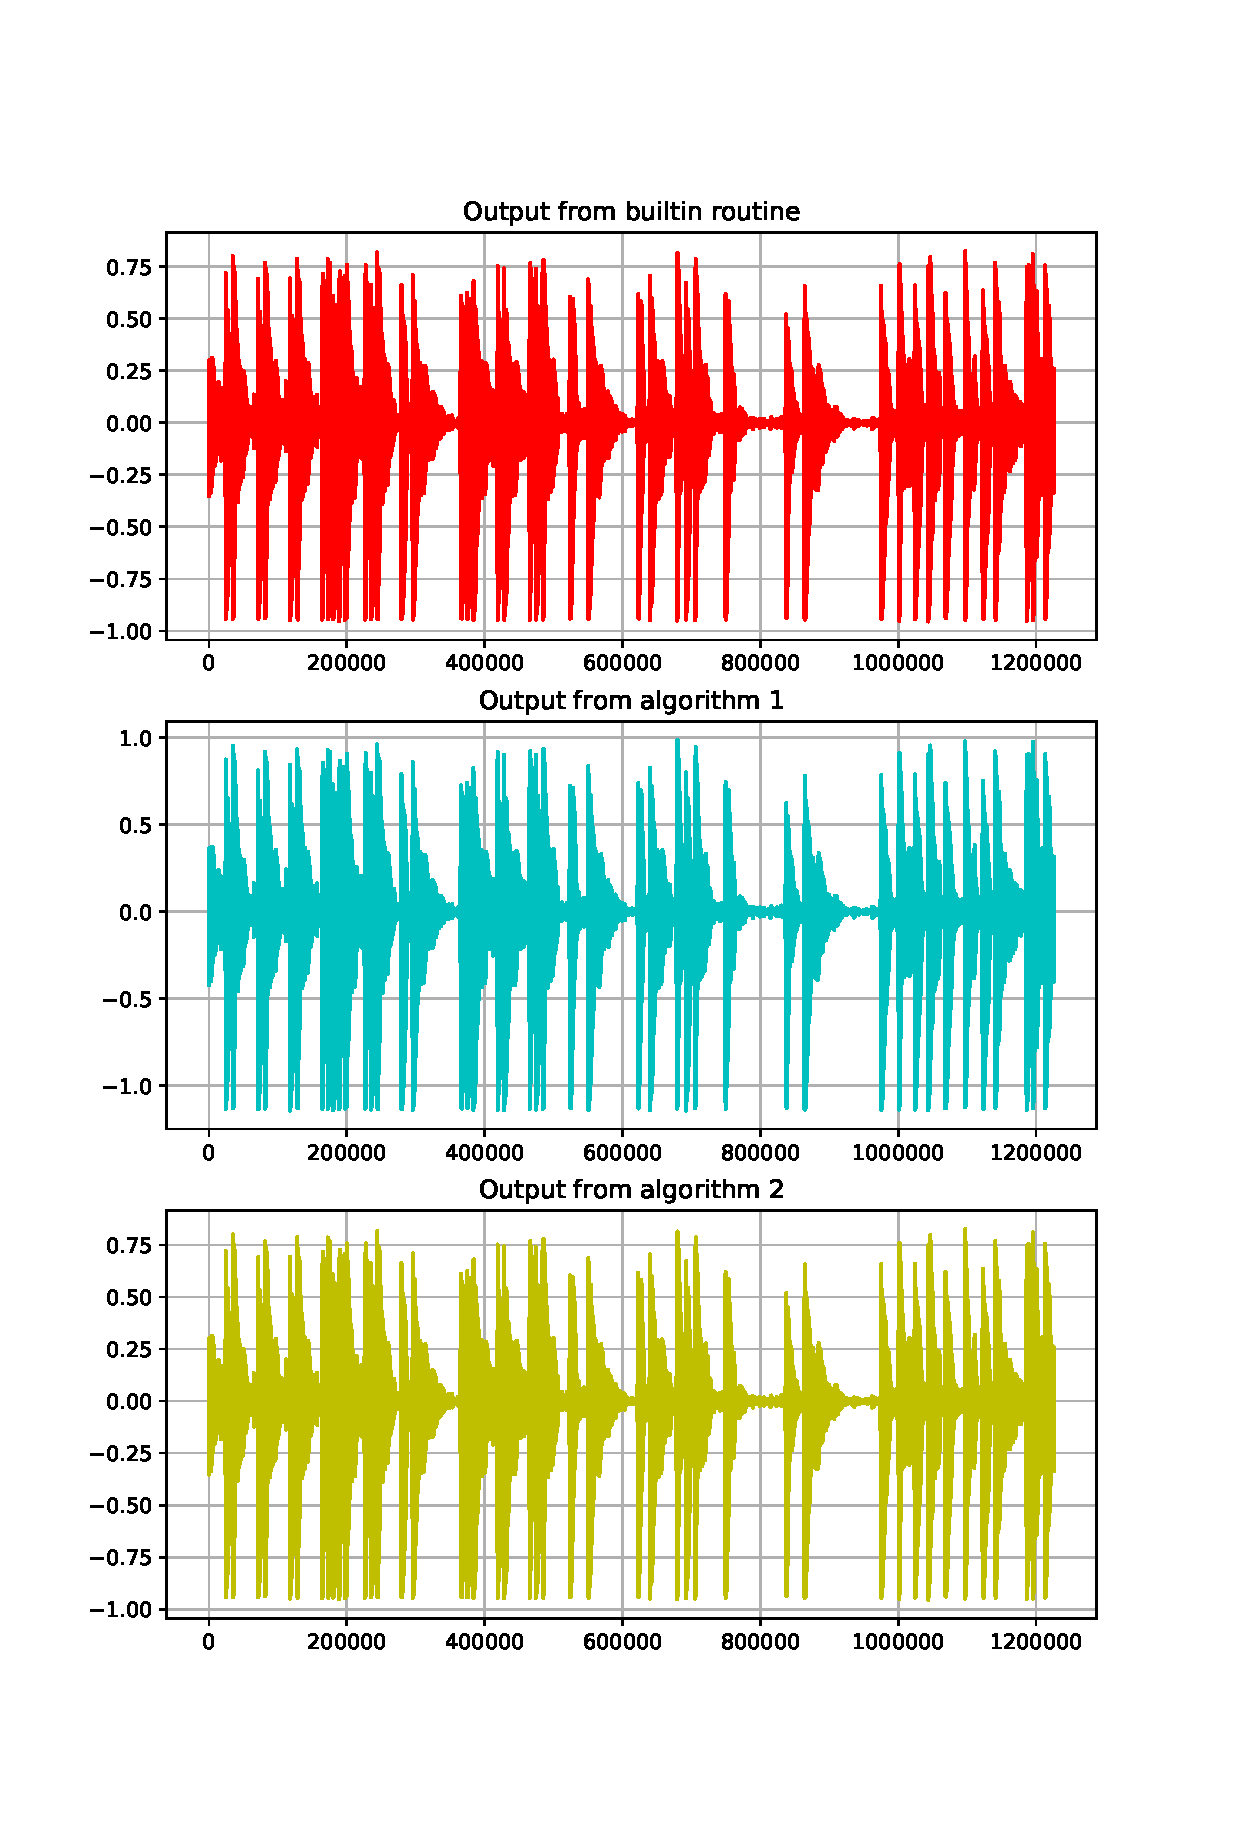
\includegraphics[width=1.2\columnwidth]{./figs/ee18btech11038_time.eps}
\caption{Time domain response}
\label{fig:Figure1}
\end{figure}
\\
\begin{figure}[!h]
\centering
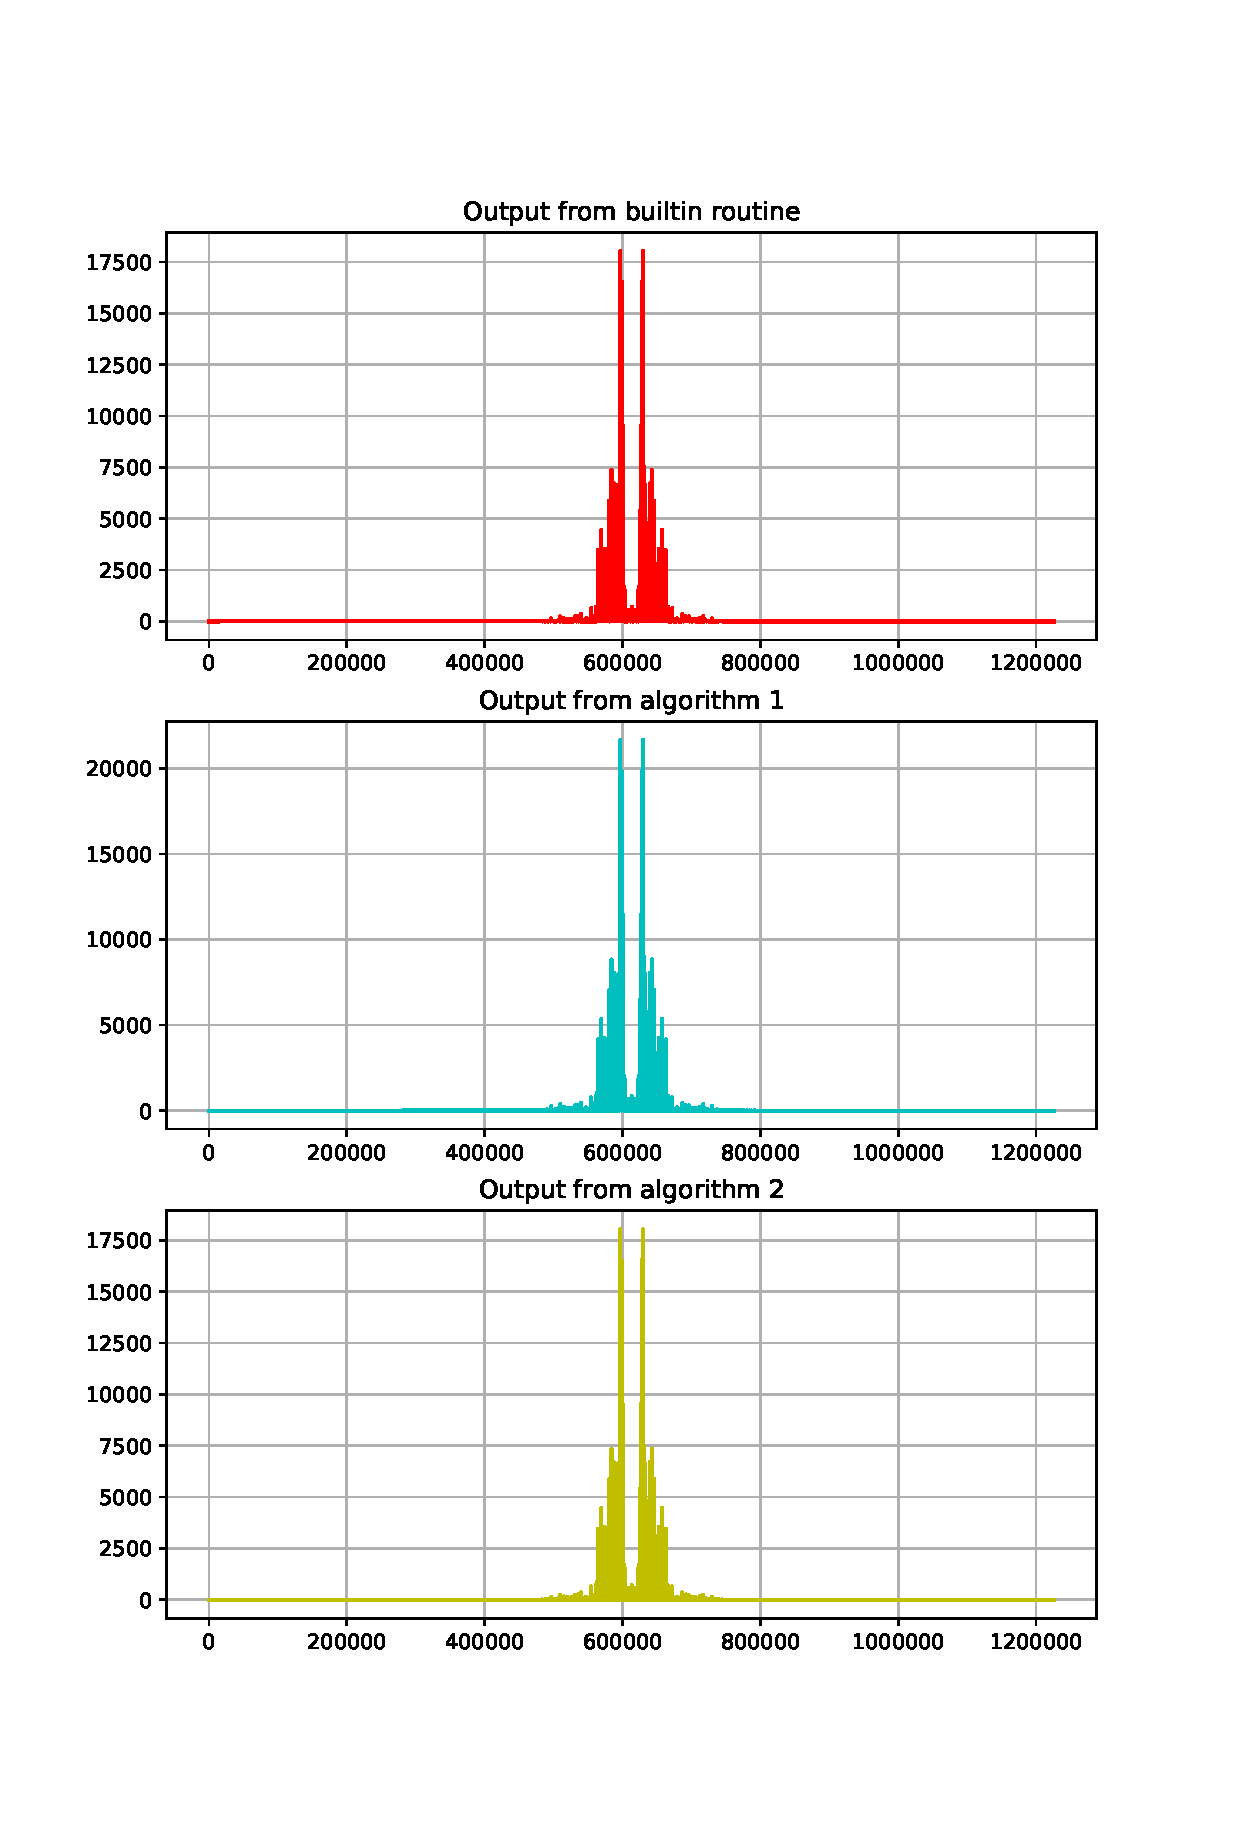
\includegraphics[width=1.2\columnwidth]{./figs/ee18btech11038_freq.eps}
\caption{Frequency domain response}
\label{fig:Figure2}
\end{figure}
\end{document}